% Options for packages loaded elsewhere
\PassOptionsToPackage{unicode}{hyperref}
\PassOptionsToPackage{hyphens}{url}
%
\documentclass[
]{article}
\usepackage{amsmath,amssymb}
\usepackage{iftex}
\ifPDFTeX
  \usepackage[T1]{fontenc}
  \usepackage[utf8]{inputenc}
  \usepackage{textcomp} % provide euro and other symbols
\else % if luatex or xetex
  \usepackage{unicode-math} % this also loads fontspec
  \defaultfontfeatures{Scale=MatchLowercase}
  \defaultfontfeatures[\rmfamily]{Ligatures=TeX,Scale=1}
\fi
\usepackage{lmodern}
\ifPDFTeX\else
  % xetex/luatex font selection
\fi
% Use upquote if available, for straight quotes in verbatim environments
\IfFileExists{upquote.sty}{\usepackage{upquote}}{}
\IfFileExists{microtype.sty}{% use microtype if available
  \usepackage[]{microtype}
  \UseMicrotypeSet[protrusion]{basicmath} % disable protrusion for tt fonts
}{}
\makeatletter
\@ifundefined{KOMAClassName}{% if non-KOMA class
  \IfFileExists{parskip.sty}{%
    \usepackage{parskip}
  }{% else
    \setlength{\parindent}{0pt}
    \setlength{\parskip}{6pt plus 2pt minus 1pt}}
}{% if KOMA class
  \KOMAoptions{parskip=half}}
\makeatother
\usepackage{xcolor}
\usepackage[margin=1in]{geometry}
\usepackage{color}
\usepackage{fancyvrb}
\newcommand{\VerbBar}{|}
\newcommand{\VERB}{\Verb[commandchars=\\\{\}]}
\DefineVerbatimEnvironment{Highlighting}{Verbatim}{commandchars=\\\{\}}
% Add ',fontsize=\small' for more characters per line
\usepackage{framed}
\definecolor{shadecolor}{RGB}{248,248,248}
\newenvironment{Shaded}{\begin{snugshade}}{\end{snugshade}}
\newcommand{\AlertTok}[1]{\textcolor[rgb]{0.94,0.16,0.16}{#1}}
\newcommand{\AnnotationTok}[1]{\textcolor[rgb]{0.56,0.35,0.01}{\textbf{\textit{#1}}}}
\newcommand{\AttributeTok}[1]{\textcolor[rgb]{0.13,0.29,0.53}{#1}}
\newcommand{\BaseNTok}[1]{\textcolor[rgb]{0.00,0.00,0.81}{#1}}
\newcommand{\BuiltInTok}[1]{#1}
\newcommand{\CharTok}[1]{\textcolor[rgb]{0.31,0.60,0.02}{#1}}
\newcommand{\CommentTok}[1]{\textcolor[rgb]{0.56,0.35,0.01}{\textit{#1}}}
\newcommand{\CommentVarTok}[1]{\textcolor[rgb]{0.56,0.35,0.01}{\textbf{\textit{#1}}}}
\newcommand{\ConstantTok}[1]{\textcolor[rgb]{0.56,0.35,0.01}{#1}}
\newcommand{\ControlFlowTok}[1]{\textcolor[rgb]{0.13,0.29,0.53}{\textbf{#1}}}
\newcommand{\DataTypeTok}[1]{\textcolor[rgb]{0.13,0.29,0.53}{#1}}
\newcommand{\DecValTok}[1]{\textcolor[rgb]{0.00,0.00,0.81}{#1}}
\newcommand{\DocumentationTok}[1]{\textcolor[rgb]{0.56,0.35,0.01}{\textbf{\textit{#1}}}}
\newcommand{\ErrorTok}[1]{\textcolor[rgb]{0.64,0.00,0.00}{\textbf{#1}}}
\newcommand{\ExtensionTok}[1]{#1}
\newcommand{\FloatTok}[1]{\textcolor[rgb]{0.00,0.00,0.81}{#1}}
\newcommand{\FunctionTok}[1]{\textcolor[rgb]{0.13,0.29,0.53}{\textbf{#1}}}
\newcommand{\ImportTok}[1]{#1}
\newcommand{\InformationTok}[1]{\textcolor[rgb]{0.56,0.35,0.01}{\textbf{\textit{#1}}}}
\newcommand{\KeywordTok}[1]{\textcolor[rgb]{0.13,0.29,0.53}{\textbf{#1}}}
\newcommand{\NormalTok}[1]{#1}
\newcommand{\OperatorTok}[1]{\textcolor[rgb]{0.81,0.36,0.00}{\textbf{#1}}}
\newcommand{\OtherTok}[1]{\textcolor[rgb]{0.56,0.35,0.01}{#1}}
\newcommand{\PreprocessorTok}[1]{\textcolor[rgb]{0.56,0.35,0.01}{\textit{#1}}}
\newcommand{\RegionMarkerTok}[1]{#1}
\newcommand{\SpecialCharTok}[1]{\textcolor[rgb]{0.81,0.36,0.00}{\textbf{#1}}}
\newcommand{\SpecialStringTok}[1]{\textcolor[rgb]{0.31,0.60,0.02}{#1}}
\newcommand{\StringTok}[1]{\textcolor[rgb]{0.31,0.60,0.02}{#1}}
\newcommand{\VariableTok}[1]{\textcolor[rgb]{0.00,0.00,0.00}{#1}}
\newcommand{\VerbatimStringTok}[1]{\textcolor[rgb]{0.31,0.60,0.02}{#1}}
\newcommand{\WarningTok}[1]{\textcolor[rgb]{0.56,0.35,0.01}{\textbf{\textit{#1}}}}
\usepackage{graphicx}
\makeatletter
\def\maxwidth{\ifdim\Gin@nat@width>\linewidth\linewidth\else\Gin@nat@width\fi}
\def\maxheight{\ifdim\Gin@nat@height>\textheight\textheight\else\Gin@nat@height\fi}
\makeatother
% Scale images if necessary, so that they will not overflow the page
% margins by default, and it is still possible to overwrite the defaults
% using explicit options in \includegraphics[width, height, ...]{}
\setkeys{Gin}{width=\maxwidth,height=\maxheight,keepaspectratio}
% Set default figure placement to htbp
\makeatletter
\def\fps@figure{htbp}
\makeatother
\setlength{\emergencystretch}{3em} % prevent overfull lines
\providecommand{\tightlist}{%
  \setlength{\itemsep}{0pt}\setlength{\parskip}{0pt}}
\setcounter{secnumdepth}{-\maxdimen} % remove section numbering
\ifLuaTeX
  \usepackage{selnolig}  % disable illegal ligatures
\fi
\usepackage{bookmark}
\IfFileExists{xurl.sty}{\usepackage{xurl}}{} % add URL line breaks if available
\urlstyle{same}
\hypersetup{
  hidelinks,
  pdfcreator={LaTeX via pandoc}}

\author{}
\date{\vspace{-2.5em}}

\begin{document}

\section{Prosjekt Titanic
overlevelse}\label{prosjekt-titanic-overlevelse}

\subsubsection{Tobias Windingstad og Ørjan
Hammer}\label{tobias-windingstad-og-uxf8rjan-hammer}

\subsubsection{Introduksjon til
oppgaven:}\label{introduksjon-til-oppgaven}

I denne oppgaven skal vi benytte et datasett fra Kaggle.com, som
inneholder informasjon om passasjerene på Titanic -- historiens mest
kjente skipsforlis. Natt til 15. april 1912 sank Titanic etter å ha
kollidert med et isfjell i Nord-Atlanteren. Datasettet gir oss
informasjon om blant annet passasjerenes alder, kjønn, klasse,
billettpris og avreisested.

Målet med prosjektet er å anvende maskinlæring for å forutsi hvilke
faktorer som hadde størst betydning for overlevelse. Vi skal trene en
modell som kan forutsi om en gitt passasjer ville ha overlevd ulykken.
Vi vil analysere variabler og deres innvirkning på overlevelse, og til
slutt bygge en prediksjonsmodell som kan teste ulike hypotetiske
scenarier.

Prosjektet er skrevet i R Markdown, hvor vi benytter både R og ulike
maskinlæringsbiblioteker for å gjennomføre analysen og prediksjonen.
Gjennom prosjektet vil vi også vurdere modellens ytelse og mulige
forbedringer for å øke prediksjonens presisjon.

\subsubsection{Dependencies}\label{dependencies}

\begin{Shaded}
\begin{Highlighting}[]
\NormalTok{dependencies }\OtherTok{\textless{}{-}} \FunctionTok{c}\NormalTok{(}\StringTok{"tidyverse"}\NormalTok{, }\StringTok{"readr"}\NormalTok{, }\StringTok{"rsample"}\NormalTok{, }\StringTok{"tidymodels"}\NormalTok{, }\StringTok{"recipes"}\NormalTok{, }\StringTok{"glmnet"}\NormalTok{, }\StringTok{"ranger"}\NormalTok{)}
\ControlFlowTok{for}\NormalTok{ (pkg }\ControlFlowTok{in}\NormalTok{ dependencies) \{}
  \ControlFlowTok{if}\NormalTok{ (}\SpecialCharTok{!}\FunctionTok{require}\NormalTok{(pkg, }\AttributeTok{character.only =} \ConstantTok{TRUE}\NormalTok{)) \{}
    \FunctionTok{install.packages}\NormalTok{(pkg)}
\NormalTok{  \}}
  \FunctionTok{library}\NormalTok{(pkg, }\AttributeTok{character.only =} \ConstantTok{TRUE}\NormalTok{)}
\NormalTok{\}}
\end{Highlighting}
\end{Shaded}

\subsubsection{Filer}\label{filer}

\begin{Shaded}
\begin{Highlighting}[]
\FunctionTok{source}\NormalTok{(}\StringTok{"../code/wrangling/wrangling.R"}\NormalTok{)}
\FunctionTok{source}\NormalTok{(}\StringTok{"../code/models/model\_data.R"}\NormalTok{)}
\FunctionTok{source}\NormalTok{(}\StringTok{"../code/models/models.R"}\NormalTok{)}
\end{Highlighting}
\end{Shaded}

\subsubsection{Data wrangling:}\label{data-wrangling}

Data wrangling er prosessen med å forberede, rense og strukturere data
for analyse (Kilde). I dette prosjektet håndterer vi flere viktige
aspekter ved datasettet for å sikre at det er klart for modellering. Her
er hva vi gjør i koden:

\begin{Shaded}
\begin{Highlighting}[]
\NormalTok{  data }\OtherTok{\textless{}{-}} \FunctionTok{wrangle\_data}\NormalTok{()}
\NormalTok{  na\_data }\OtherTok{\textless{}{-}} \FunctionTok{wrangle\_data}\NormalTok{(}\AttributeTok{na =} \ConstantTok{TRUE}\NormalTok{)}
\end{Highlighting}
\end{Shaded}

\paragraph{1. Behandling av manglende verdier
(NA)}\label{behandling-av-manglende-verdier-na}

\subparagraph{Avreisehavn:}\label{avreisehavn}

To av passasjerene mangler avreisehavn. Siden begge disse passasjerene
har reist med førsteklasse og betalt samme pris finner vi
gjennomsnittsprisen for alle førsteklasse-reisende for hver havn. Vi
setter så avreisehavnen for de to passasjerene til den havnen som
korrelerer best med prisen de har betalt.

\begin{center}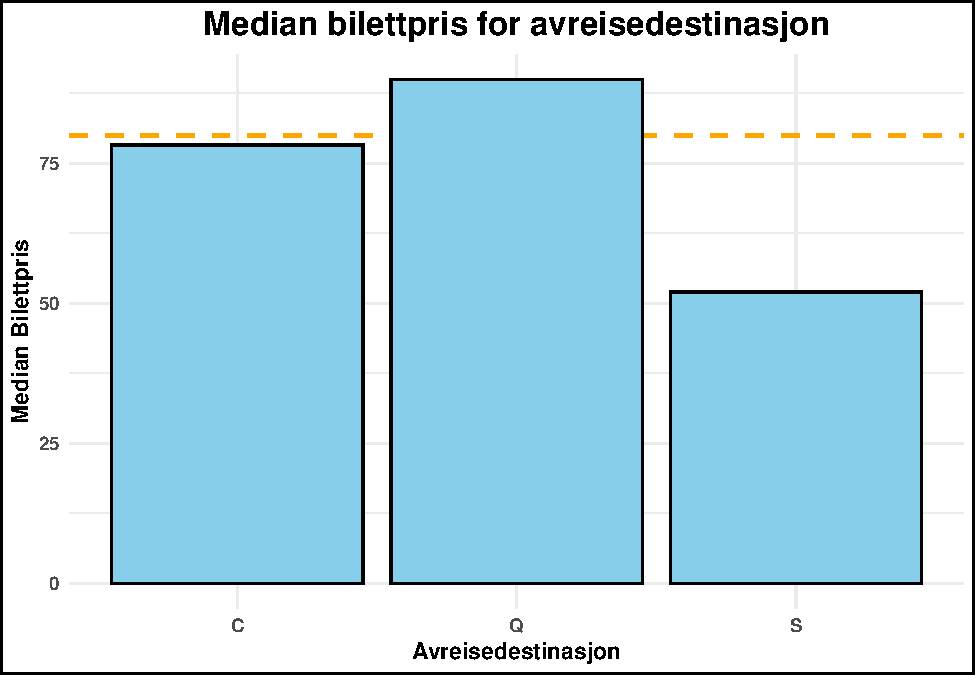
\includegraphics{presentation_files/figure-latex/unnamed-chunk-4-1} \end{center}

\section{}\label{section}

\subparagraph{Alder}\label{alder}

For passasjerer med manglende alder, bruker vi en median-alder som
standard, med en ekstra detalj for personer som reiste med søsken eller
ektefelle (SibSp \textgreater{} 0), men ikke med barn eller foreldre
(Parch == 0). I slike tilfeller bruker vi gjennomsnittsalderen for
personer med samme etternavn (antatt å være søsken eller ektefeller).
Dette gir mange av de reisende medianalder, men vi mener at ved å legge
til denne behandlingen vil vi kunne ha noe sterkere antakelser om
alderen til noen av passasjerene.

\begin{Shaded}
\begin{Highlighting}[]
\NormalTok{handle\_na\_age }\OtherTok{\textless{}{-}} \ControlFlowTok{function}\NormalTok{(data) \{}
\NormalTok{  median\_age }\OtherTok{\textless{}{-}} \FunctionTok{median}\NormalTok{(data}\SpecialCharTok{$}\NormalTok{Age, }\AttributeTok{na.rm =} \ConstantTok{TRUE}\NormalTok{)}
\NormalTok{  data }\OtherTok{\textless{}{-}}\NormalTok{ data }\SpecialCharTok{\%\textgreater{}\%}
    \FunctionTok{mutate}\NormalTok{(}\AttributeTok{Age =} \FunctionTok{ifelse}\NormalTok{(}\FunctionTok{is.na}\NormalTok{(Age), }\FunctionTok{ifelse}\NormalTok{((SibSp }\SpecialCharTok{\textgreater{}} \DecValTok{0}\NormalTok{) }\SpecialCharTok{\&}\NormalTok{ (Parch }\SpecialCharTok{==} \DecValTok{0}\NormalTok{), }\FunctionTok{getSibSpAge}\NormalTok{(Name, data), median\_age), Age))}
  \FunctionTok{return}\NormalTok{(data)}
\NormalTok{\}}

\NormalTok{getSibSpAge }\OtherTok{\textless{}{-}} \ControlFlowTok{function}\NormalTok{(name, data) \{}
\NormalTok{  last\_name }\OtherTok{\textless{}{-}} \FunctionTok{get\_last\_name}\NormalTok{(name)}
  
\NormalTok{  sib\_sp }\OtherTok{\textless{}{-}} \FunctionTok{filter}\NormalTok{(}\FunctionTok{group\_by}\NormalTok{(data, Name), }\FunctionTok{get\_last\_name}\NormalTok{(Name) }\SpecialCharTok{==}\NormalTok{ last\_name)}
  
\NormalTok{  estimated\_age }\OtherTok{\textless{}{-}} \FunctionTok{round}\NormalTok{(}\FunctionTok{mean}\NormalTok{(sib\_sp}\SpecialCharTok{$}\NormalTok{Age, }\AttributeTok{na.rm =} \ConstantTok{TRUE}\NormalTok{))}
  \FunctionTok{return}\NormalTok{ (estimated\_age)}
\NormalTok{\}}

\NormalTok{get\_last\_name }\OtherTok{\textless{}{-}} \ControlFlowTok{function}\NormalTok{(name) \{}
\NormalTok{  last\_name }\OtherTok{\textless{}{-}} \FunctionTok{strsplit}\NormalTok{(name, }\StringTok{\textquotesingle{},\textquotesingle{}}\NormalTok{)[[}\DecValTok{1}\NormalTok{]][}\DecValTok{1}\NormalTok{]}
  \FunctionTok{return}\NormalTok{ (last\_name)}
\NormalTok{\}}
\end{Highlighting}
\end{Shaded}

\paragraph{2. Ekstrahere tittel}\label{ekstrahere-tittel}

Vi ønsket å isolere tittelen fra navnet og legge den til i en egen
kolonne. Vår teori er at dette kan gjøre dataen mer tilpasset
maskinlæring ettersom tittelen kan være en indikator på faktorer som
sivilstatus, alder eller sosioøkonomisk status.

\paragraph{3. Fjerne irrelevante og manglende
variabler}\label{fjerne-irrelevante-og-manglende-variabler}

For å redusere kompleksiteten i datasettet fjerner vi kolonnen Cabin
ettersom den har svært mange i datasettet som ikke hadde denne
variabelen. Vi så først på muligheten for at det var en tydelig
sammenheng mellom Pclass og Cabin ved bruk av en Chi-Squared. Det var
tydelig at passasjerer i Pclass 1 var konsentrert i A, B, C og D
kabiner, men ettersom det er svært lite data på hvor de resterende
reisende bodde, ville vi ikke gjøre noen generalisering rundt dette.
Name, Ticket og PassangerId er alle individuelle verdier som ikke vil ha
noen påvirkning på modellene så vi fjernet disse.

Gjennom denne prosessen sørger vi for at datasettet er renere, mer
konsistente og at de manglende variablene er håndtert.

\subsubsection{Kan vise helper-functions som ikke kan kjøres fra
r-markdown siden wrangle\_data() allerede gjør det.
F.eks.}\label{kan-vise-helper-functions-som-ikke-kan-kjuxf8res-fra-r-markdown-siden-wrangle_data-allerede-gjuxf8r-det.-f.eks.}

\begin{Shaded}
\begin{Highlighting}[]
\NormalTok{get\_titles }\OtherTok{\textless{}{-}} \ControlFlowTok{function}\NormalTok{(data)\{}
\NormalTok{  data }\OtherTok{\textless{}{-}}\NormalTok{ data }\SpecialCharTok{\%\textgreater{}\%}
    \FunctionTok{mutate}\NormalTok{(}\AttributeTok{Title =} \FunctionTok{sub}\NormalTok{(}\StringTok{".*,}\SpecialCharTok{\textbackslash{}\textbackslash{}}\StringTok{s*(}\SpecialCharTok{\textbackslash{}\textbackslash{}}\StringTok{w+)}\SpecialCharTok{\textbackslash{}\textbackslash{}}\StringTok{..*"}\NormalTok{, }\StringTok{"}\SpecialCharTok{\textbackslash{}\textbackslash{}}\StringTok{1"}\NormalTok{, Name))}
  \FunctionTok{return}\NormalTok{(data)}
\NormalTok{\}}
\end{Highlighting}
\end{Shaded}

\subsubsection{Lag dummy-data og initial
split}\label{lag-dummy-data-og-initial-split}

\begin{Shaded}
\begin{Highlighting}[]
\NormalTok{model\_data }\OtherTok{\textless{}{-}} \FunctionTok{create\_dummy\_data}\NormalTok{(data)}
\NormalTok{t\_train }\OtherTok{\textless{}{-}}\NormalTok{ model\_data}\SpecialCharTok{$}\NormalTok{t\_train}
\NormalTok{t\_test }\OtherTok{\textless{}{-}}\NormalTok{ model\_data}\SpecialCharTok{$}\NormalTok{t\_test}
\end{Highlighting}
\end{Shaded}

\subsubsection{OLS model}\label{ols-model}

\begin{Shaded}
\begin{Highlighting}[]
\NormalTok{ols\_model }\OtherTok{\textless{}{-}} \FunctionTok{linear\_regression\_model}\NormalTok{(t\_train)}
  \FunctionTok{print}\NormalTok{(}\StringTok{"Trained OLS model:"}\NormalTok{)}
  \FunctionTok{print}\NormalTok{(}\FunctionTok{summary}\NormalTok{(ols\_model))}
  \FunctionTok{print}\NormalTok{(}\FunctionTok{alias}\NormalTok{(ols\_model}\SpecialCharTok{$}\NormalTok{fit))}

\NormalTok{  ols\_pred }\OtherTok{\textless{}{-}} \FunctionTok{predict}\NormalTok{(ols\_model, }\AttributeTok{new\_data =}\NormalTok{ t\_test) }\SpecialCharTok{\%\textgreater{}\%} \FunctionTok{pull}\NormalTok{(.pred)}
\end{Highlighting}
\end{Shaded}

\subsubsection{LASSO model}\label{lasso-model}

\begin{Shaded}
\begin{Highlighting}[]
\NormalTok{lso\_model }\OtherTok{\textless{}{-}} \FunctionTok{lasso\_model}\NormalTok{(t\_train)}
  \FunctionTok{print}\NormalTok{(}\StringTok{"Trained LASSO model:"}\NormalTok{)}
  \FunctionTok{print}\NormalTok{(}\FunctionTok{summary}\NormalTok{(lso\_model))}

\NormalTok{  lso\_pred }\OtherTok{\textless{}{-}} \FunctionTok{predict}\NormalTok{(lso\_model, }\AttributeTok{new\_data =}\NormalTok{ t\_test) }\SpecialCharTok{\%\textgreater{}\%} \FunctionTok{pull}\NormalTok{(.pred)}
\end{Highlighting}
\end{Shaded}

\subsubsection{Random Forest model}\label{random-forest-model}

\begin{Shaded}
\begin{Highlighting}[]
\NormalTok{rf\_model }\OtherTok{\textless{}{-}} \FunctionTok{random\_forest\_model}\NormalTok{(t\_train)}
  \FunctionTok{print}\NormalTok{(}\StringTok{"Trained random forest model:"}\NormalTok{)}
  \FunctionTok{print}\NormalTok{(}\FunctionTok{summary}\NormalTok{(rf\_model))}

\NormalTok{  rf\_pred }\OtherTok{\textless{}{-}} \FunctionTok{predict}\NormalTok{(rf\_model, }\AttributeTok{new\_data =}\NormalTok{ t\_test) }\SpecialCharTok{\%\textgreater{}\%} \FunctionTok{pull}\NormalTok{(.pred)}
\end{Highlighting}
\end{Shaded}

\subsubsection{Gradient Boosting Tree
model}\label{gradient-boosting-tree-model}

\begin{Shaded}
\begin{Highlighting}[]
\NormalTok{xgb\_model }\OtherTok{\textless{}{-}} \FunctionTok{xgboost\_model}\NormalTok{(t\_train)}
  \FunctionTok{print}\NormalTok{(}\StringTok{"Trained Gradient Boosting Tree model:"}\NormalTok{)}
  \FunctionTok{print}\NormalTok{(}\FunctionTok{summary}\NormalTok{(xgb\_model))}
  
\NormalTok{  xgb\_pred }\OtherTok{\textless{}{-}} \FunctionTok{predict}\NormalTok{(xgb\_model, }\AttributeTok{new\_data =}\NormalTok{ t\_test) }\SpecialCharTok{\%\textgreater{}\%} \FunctionTok{pull}\NormalTok{(.pred)}
\end{Highlighting}
\end{Shaded}

\begin{Shaded}
\begin{Highlighting}[]
\NormalTok{errs }\OtherTok{\textless{}{-}} \FunctionTok{tibble}\NormalTok{(}
    \AttributeTok{Actual =}\NormalTok{ t\_test}\SpecialCharTok{$}\NormalTok{Survived,}
    \AttributeTok{OLS\_errors =}\NormalTok{ Actual }\SpecialCharTok{{-}}\NormalTok{ ols\_pred,}
    \AttributeTok{LSO\_errors =}\NormalTok{ Actual }\SpecialCharTok{{-}}\NormalTok{ lso\_pred,}
    \AttributeTok{RF\_errors =}\NormalTok{ Actual }\SpecialCharTok{{-}}\NormalTok{ rf\_pred,}
    \AttributeTok{XGB\_errors =}\NormalTok{ Actual }\SpecialCharTok{{-}}\NormalTok{ xgb\_pred,}
\NormalTok{  ) }
\end{Highlighting}
\end{Shaded}

\subsubsection{Kalkulere MSE og
Accuracy}\label{kalkulere-mse-og-accuracy}

\begin{Shaded}
\begin{Highlighting}[]
\NormalTok{mse\_ols }\OtherTok{\textless{}{-}} \FunctionTok{mean}\NormalTok{(errs}\SpecialCharTok{$}\NormalTok{OLS\_errors}\SpecialCharTok{\^{}}\DecValTok{2}\NormalTok{)}
\FunctionTok{print}\NormalTok{(}\FunctionTok{paste}\NormalTok{(}\StringTok{"MSE OLS: "}\NormalTok{, mse\_ols))}
  
\NormalTok{mse\_lso }\OtherTok{\textless{}{-}} \FunctionTok{mean}\NormalTok{(errs}\SpecialCharTok{$}\NormalTok{LSO\_errors}\SpecialCharTok{\^{}}\DecValTok{2}\NormalTok{)}
\FunctionTok{print}\NormalTok{(}\FunctionTok{paste}\NormalTok{(}\StringTok{"MSE LSO: "}\NormalTok{, mse\_lso))}
  
\NormalTok{mse\_rf }\OtherTok{\textless{}{-}} \FunctionTok{mean}\NormalTok{(errs}\SpecialCharTok{$}\NormalTok{RF\_errors}\SpecialCharTok{\^{}}\DecValTok{2}\NormalTok{)}
\FunctionTok{print}\NormalTok{(}\FunctionTok{paste}\NormalTok{(}\StringTok{"MSE RF: "}\NormalTok{, mse\_rf))}
  
\NormalTok{mse\_xgb }\OtherTok{\textless{}{-}} \FunctionTok{mean}\NormalTok{(errs}\SpecialCharTok{$}\NormalTok{XGB\_errors}\SpecialCharTok{\^{}}\DecValTok{2}\NormalTok{)}
\FunctionTok{print}\NormalTok{(}\FunctionTok{paste}\NormalTok{(}\StringTok{"MSE XGB: "}\NormalTok{, mse\_xgb))}
  
\NormalTok{acc\_ols }\OtherTok{=}  \FunctionTok{sum}\NormalTok{((errs}\SpecialCharTok{$}\NormalTok{OLS }\SpecialCharTok{\textgreater{}} \FloatTok{0.499}\NormalTok{) }\SpecialCharTok{==}\NormalTok{ errs}\SpecialCharTok{$}\NormalTok{Actual) }\SpecialCharTok{/} \FunctionTok{length}\NormalTok{(errs}\SpecialCharTok{$}\NormalTok{Actual)}
\NormalTok{acc\_lso }\OtherTok{=} \FunctionTok{sum}\NormalTok{((errs}\SpecialCharTok{$}\NormalTok{LSO }\SpecialCharTok{\textgreater{}} \FloatTok{0.499}\NormalTok{) }\SpecialCharTok{==}\NormalTok{ errs}\SpecialCharTok{$}\NormalTok{Actual) }\SpecialCharTok{/} \FunctionTok{length}\NormalTok{(errs}\SpecialCharTok{$}\NormalTok{Actual)}
\NormalTok{acc\_rf }\OtherTok{=} \FunctionTok{sum}\NormalTok{((errs}\SpecialCharTok{$}\NormalTok{RF }\SpecialCharTok{\textgreater{}} \FloatTok{0.499}\NormalTok{) }\SpecialCharTok{==}\NormalTok{ errs}\SpecialCharTok{$}\NormalTok{Actual) }\SpecialCharTok{/} \FunctionTok{length}\NormalTok{(errs}\SpecialCharTok{$}\NormalTok{Actual)}
\NormalTok{acc\_xgb }\OtherTok{=} \FunctionTok{sum}\NormalTok{((errs}\SpecialCharTok{$}\NormalTok{XGB }\SpecialCharTok{\textgreater{}} \FloatTok{0.499}\NormalTok{) }\SpecialCharTok{==}\NormalTok{ errs}\SpecialCharTok{$}\NormalTok{Actual) }\SpecialCharTok{/} \FunctionTok{length}\NormalTok{(errs}\SpecialCharTok{$}\NormalTok{Actual)}
  
\NormalTok{accuracy }\OtherTok{\textless{}{-}} \FunctionTok{tibble}\NormalTok{(}
  \AttributeTok{osl =}\NormalTok{ acc\_ols,}
  \AttributeTok{lso =}\NormalTok{ acc\_lso,}
  \AttributeTok{rf =}\NormalTok{ acc\_rf,}
  \AttributeTok{xgb =}\NormalTok{ acc\_xgb}
\NormalTok{)}
\FunctionTok{print}\NormalTok{(accuracy)}
\end{Highlighting}
\end{Shaded}


\end{document}
